\documentclass[border=10pt]{standalone}
\usepackage[svgnames]{xcolor}
\usepackage{amsmath}
\usepackage{pgfplots}
\pgfplotsset{compat=newest}
\usepackage[sfdefault]{FiraSans}
\usepackage{FiraMono}
\renewcommand*\familydefault{\sfdefault}
\begin{document}
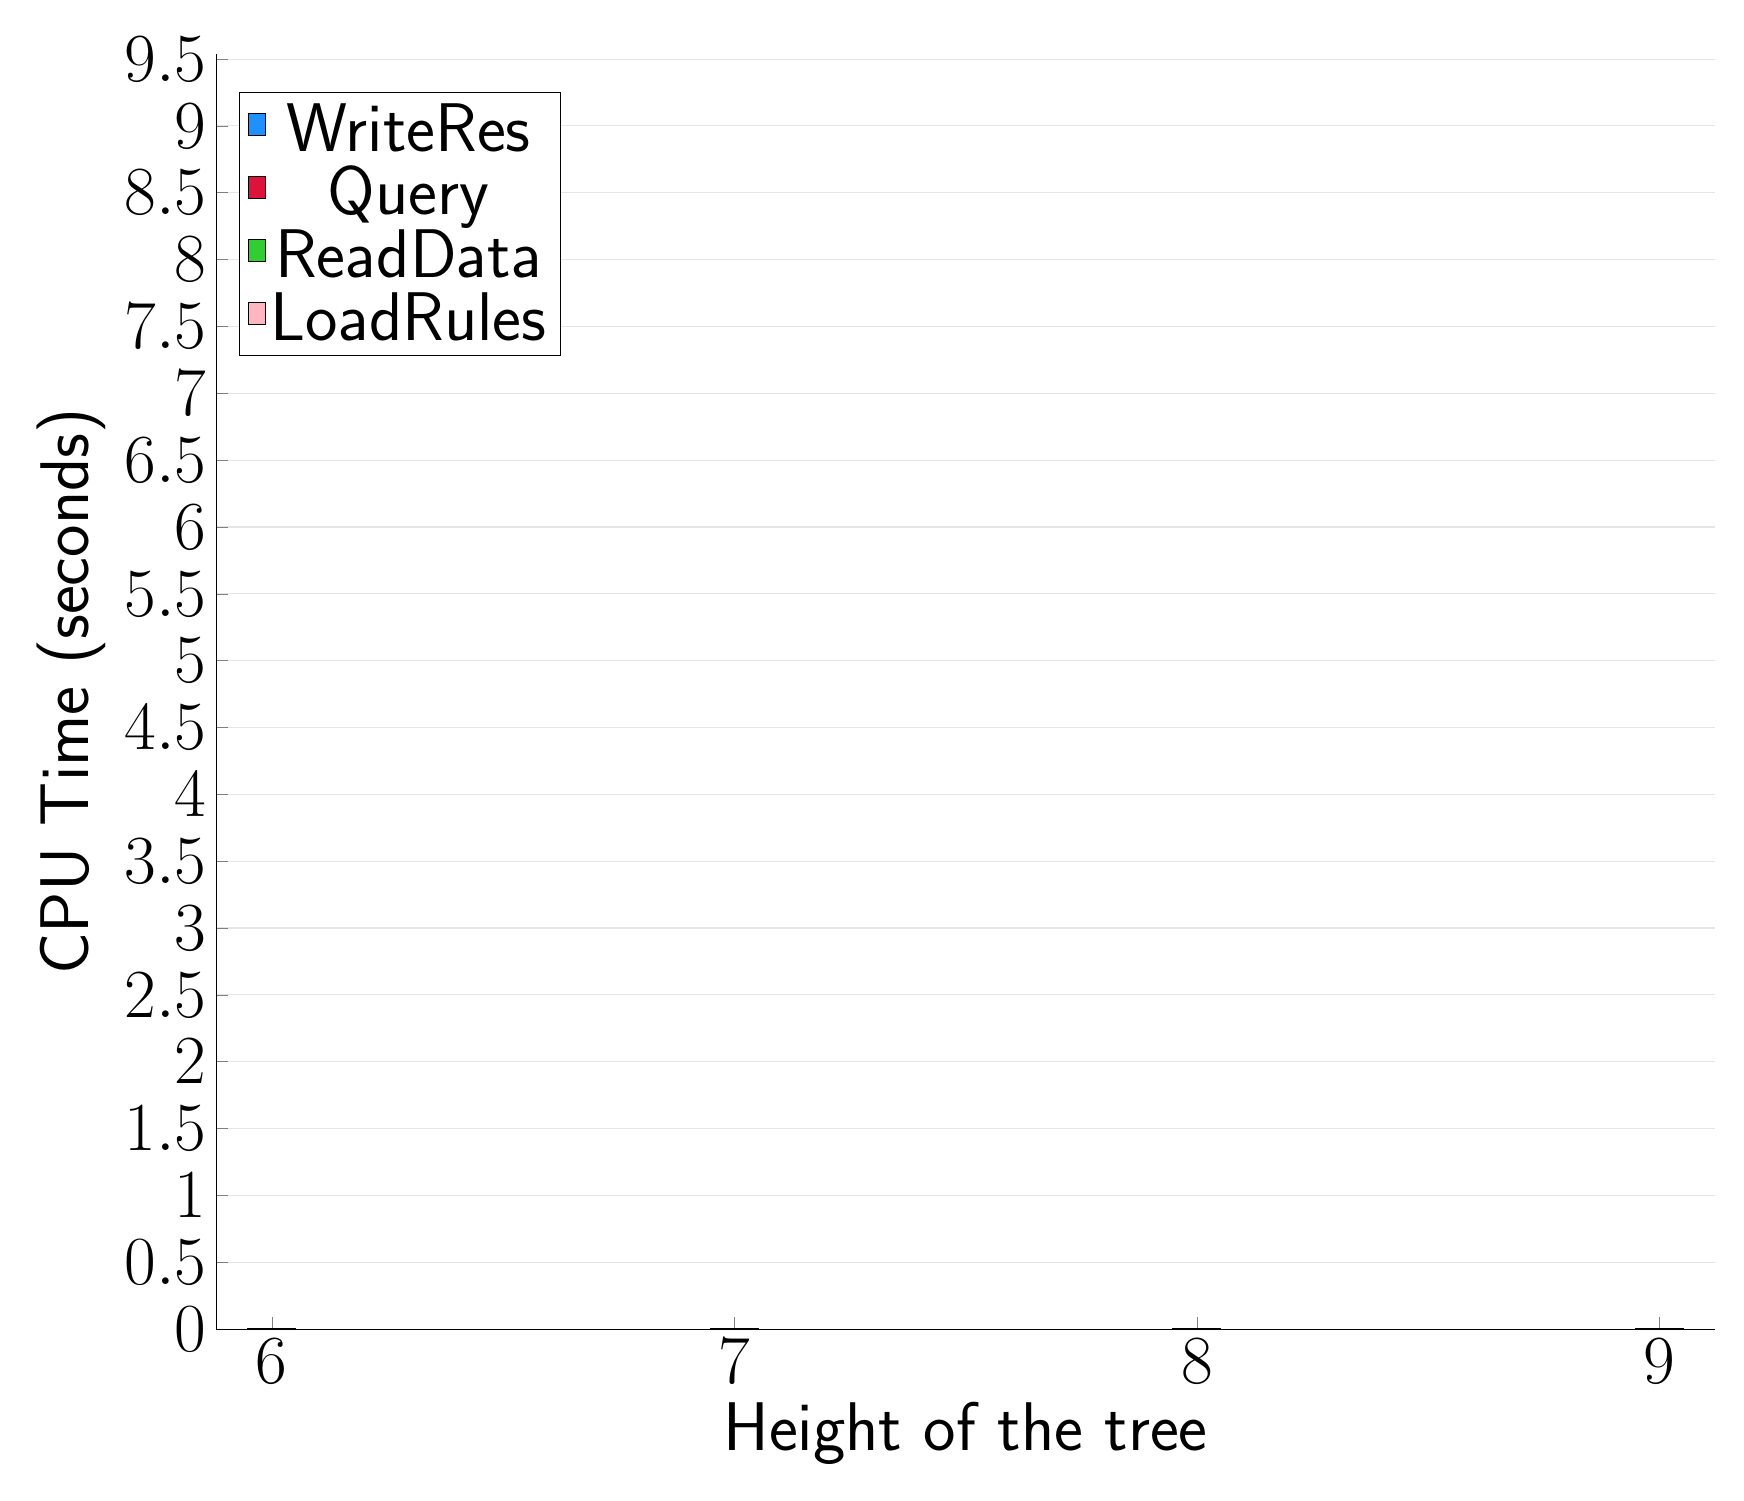
\begin{tikzpicture}
\begin{axis}[
   ybar stacked,
   width=1.7\textwidth,
   bar width=0.6cm,
   ymajorgrids, tick align=inside,
   major grid style={draw=gray!20},
   xtick=data,
   ymin=0, ymax=9.54,
   axis x line*=bottom,
   axis y line*=left,
   enlarge x limits=0.04,
   legend style={
       at={(0.23, 0.97)},
       anchor=north east,
       legend columns=1,
       font=\Huge,
   },
   ylabel={CPU Time (seconds)},
   xlabel={Height of the tree},
   label style={font=\Huge},
   tick label style={font=\Huge},
]
\addlegendimage{fill=DodgerBlue, draw=black, line width=0.2pt}
\addlegendentry{WriteRes}
\addlegendimage{fill=Crimson, draw=black, line width=0.2pt}
\addlegendentry{Query}
\addlegendimage{fill=LimeGreen, draw=black, line width=0.2pt}
\addlegendentry{ReadData}
\addlegendimage{fill=LightPink, draw=black, line width=0.2pt}
\addlegendentry{LoadRules}
\addplot +[fill=LightPink, draw=black, line width=0.55pt] coordinates {
(6, 0.0005624000000000002)
(7, 0.0005533999999999997)
(8, 0.0005548)
(8, 0.0005524000000000002)
(8, 0.0005488000000000001)
(9, 0.0005541999999999997)
(9, 0.0005540000000000002)
(9, 0.0005528)
(9, 0.0005559999999999999)
(9, 0.0005564)
};
\addplot +[fill=LimeGreen, draw=black, line width=0.55pt] coordinates {
(6, 0.00017360000000000018)
(7, 0.00022059999999999962)
(8, 0.0003200000000000002)
(8, 0.0003236000000000002)
(8, 0.00032360000000000017)
(9, 0.0005202000000000002)
(9, 0.0005217999999999998)
(9, 0.0005166)
(9, 0.0005339999999999999)
(9, 0.0005157999999999997)
};
\addplot +[fill=Crimson, draw=black, line width=0.55pt] coordinates {
(6, 4.739999999999989e-05)
(7, 0.00010580000000000019)
(8, 0.0002472)
(8, 0.0002459999999999998)
(8, 0.0002483999999999992)
(9, 0.0005851999999999998)
(9, 0.0005930000000000004)
(9, 0.0005911999999999998)
(9, 0.0005864000000000005)
(9, 0.0005892000000000002)
};
\addplot +[fill=DodgerBlue, draw=black, line width=0.55pt] coordinates {
(6, 7.899999999999971e-05)
(7, 0.0001003999999999998)
(8, 0.0001424)
(8, 0.00014559999999999996)
(8, 0.00013740000000000117)
(9, 0.00021380000000000018)
(9, 0.0002046)
(9, 0.00020980000000000017)
(9, 0.0002131999999999996)
(9, 0.00021899999999999958)
};
\end{axis}
\end{tikzpicture}

\end{document}
